\documentclass{beamer}
%\documentclass[handout]{beamer}
% This file is a solution template for:

% - Giving a talk on some subject.
% - The talk is between 15min and 45min long.
% - Style is ornate.

% Copyright 2004 by Till Tantau <tantau@users.sourceforge.net>.
%
% In principle, this file can be redistributed and/or modified under
% the terms of the GNU Public License, version 2.
%
% However, this file is supposed to be a template to be modified
% for your own needs. For this reason, if you use this file as a
% template and not specifically distribute it as part of a another
% package/program, I grant the extra permission to freely copy and
% modify this file as you see fit and even to delete this copyright
% notice. 

\mode<presentation>
{
  \usetheme{Montpellier}

  %\setbeamercovered{transparent}
  % or whatever (possibly just delete it)
}

\usepackage{xmpmulti} % package that defines \multiinclude

\usepackage[english]{babel}

\usepackage[latin1]{inputenc}

\usepackage{times}
\usepackage[T1]{fontenc}
% Or whatever. Note that the encoding and the font should match. If T1
% does not look nice, try deleting the line with the fontenc.

\title [Learning in repeated games] %(optional, use only with long paper titles)
{Online learning \\ in \\ repeated matrix games}

\author[Freund] % (optional, use only with lots of authors)
{Yoav Freund}
% - Give the names in the same order as the appear in the paper.
% - Use the \inst{?} command only if the authors have different
%   affiliation.

\institute[Universities of Somewhere and Elsewhere] % (optional, but mostly needed)

\subject{Machine Learning}
% This is only inserted into the PDF information catalog. Can be left
% out. 

% If you have a file called "university-logo-filename.xxx", where xxx
% is a graphic format that can be processed by latex or pdflatex,
% resp., then you can add a logo as follows:

% \pgfdeclareimage[height=0.5cm]{university-logo}{university-logo-filename}
% \logo{\pgfuseimage{university-logo}}



% Delete this, if you do not want the table of contents to pop up at
% the beginning of each subsection:
%% \AtBeginSubsection[]
%% {
%%   \begin{frame}<beamer>
%%     \frametitle{Outline}
%%     \tableofcontents[currentsection,currentsubsection]
%%   \end{frame}
%% }


% If you wish to uncover everything in a step-wise fashion, uncomment
% the following command: 

\beamerdefaultoverlayspecification{<+->}

\newcommand{\newmcommand}[2]{\newcommand{#1}{{\ifmmode {#2}\else\mbox{${#2}$}\fi}}}
\newcommand{\newmcommandi}[2]{\newcommand{#1}[1]{{\ifmmode {#2}\else\mbox{${#2}$}\fi}}}
\newcommand{\newmcommandii}[2]{\newcommand{#1}[2]{{\ifmmode {#2}\else\mbox{${#2}$}\fi}}}
\newcommand{\newmcommandiii}[2]{\newcommand{#1}[3]{{\ifmmode {#2}\else\mbox{${#2}$}\fi}}}

\newcommand{\algfnt}{\bf}

\newmcommand{\ouralg}{{\mbox{\algfnt Hedge}({\eta})}}

\newmcommand{\iter}{T}

\newfont{\cmmib}{cmmib10}
\newcommand{\boldell}{{\mbox{\cmmib \symbol{'140}}}}

\newmcommandi{\costvec}{{\boldell}^{#1}}
\newmcommandii{\cost}{{\ell}^{#1}_{#2}}

\newmcommandi{\rd}{\tilde{#1}}

\newmcommandi{\distvec}{{\bf p}^{#1}}
\newmcommandi{\rddistvec}{\rd{\bf p}^{#1}}
\newmcommandii{\dist}{{p}^{#1}_{#2}}
\newmcommandii{\rddist}{\rd{p}^{#1}_{#2}}

\newmcommandi{\bdistvec}{{\bf q}^{#1}}
\newmcommandii{\bdist}{{q}^{#1}_{#2}}

\newmcommandi{\wtvec}{{\bf w}^{#1}}
\newmcommandi{\rdwtvec}{\rd{\bf w}^{#1}}
\newmcommandii{\wt}{{w}^{#1}_{#2}}
\newmcommandii{\rdwt}{\rd{w}^{#1}_{#2}}

\newcommand{\w}[1]{\makebox[12pt]{{#1}}}
\newcommand{\Rps}{\mbox{\tt R}}
\newcommand{\rPs}{\mbox{\tt P}}
\newcommand{\rpS}{\mbox{\tt S}}
\newcommand{\rpstie}{\w{$\frac{1}{2}$}}
\newcommand{\rpswin}{\w{$0$}}
\newcommand{\rpsloss}{\w{$1$}}

\newmcommand{\decspace}{\Delta}
\newmcommand{\decsym}{\delta}
\newmcommandi{\dec}{\decsym^{#1}}
\newmcommand{\decdistsym}{\cal D}
\newmcommandi{\decdist}{{\decdistsym}^{#1}}

\newmcommand{\simpdistspace}{{\bf \cal S}}
\newmcommand{\domset}{{\rm dom}(\decdistsym)}

\newmcommand{\expdistsym}{{\cal E}}
\newmcommandii{\expdist}{{\expdistsym}^{#1}_{#2}}
\newmcommand{\expdecsym}{{\varepsilon}}
\newmcommandii{\expdec}{\expdecsym^{#1}_{#2}}

\newmcommand{\outspace}{\Omega}
\newmcommand{\outsym}{\omega}
\newmcommandi{\out}{\outsym^{#1}}

%\newmcommandii{\Dkl}{D_{\mbox{kl}}\paren{#1||#2}}
\newmcommandii{\Dkl}{{\rm {KL}}\paren{{#1}\;||\;{#2}}}

\newmcommandi{\sumwts}{\sum_{i=1}^N \wt{#1}{i}}

\newmcommand{\lossalg}{L_A}
\newmcommand{\lossouralg}{{L_{\mbox{\scriptsize\algfnt Hedge}(\eta)}}}
\newmcommand{\lossS}{{L_{\mbox{\scriptsize\algfnt S}}}}
\newmcommandi{\lossi}{L_{#1}}
\newmcommandii{\lossit}{L_{#1}^{#2}}

\newmcommandi{\upbnd}{\tilde{#1}}

\newcommand{\angles}[1]{{\left\langle {#1} \right\rangle}}
\newcommand{\paren}[1]{{\left( {#1} \right)}}
\newcommand{\abs}[1]{{\left| {#1} \right|}}
\newcommand{\ceiling}[1]{{\left\lceil {#1} \right\rceil}}

\newfont{\msym}{msbm10}
\newcommand{\real}{\mbox{\msym R}}

\newmcommand{\updatefcn}{U_\eta}

%% \newtheorem{theorem}{Theorem}	
%% \newtheorem{lemma}[theorem]{Lemma}
%% \newtheorem{corollary}[theorem]{Corollary}
%% \newtheorem{definition}{Definition}

%\newcommand{\proof}{\noindent{\bf Proof:} }
%\newcommand{\example}[1]{{\em Example #1.} }
%\newcommand{\qed}{\rule{0.7em}{0.7em}}

\newcommand{\WeakAlg}{\mbox{\algfnt WeakLearn}}
\newcommand{\Boost}{\mbox{\algfnt AdaBoost}}
\newcommand{\EX}{\mbox{\bf EX}}
\newmcommand{\hf}{h_{{f}}}
\newmcommand{\rdhf}{\rd{h}_{{f}}}
\newmcommand{\hfT}{h^T_{{f}}}
\newmcommand{\ranh}{{b}}

\newmcommand{\conclass}{{\cal C}}

\newmcommand{\badvec}{{\bf b}}
\newmcommandi{\bad}{{b}_{#1}}

%%%%%%%% New commands defined for the game-playing paper

\newmcommand{\hedge}{\algfnt Hedge}
\newmcommand{\play}{\algfnt Play}
\newmcommandi{\Glossvec}{{\bg y}^{#1}}
\newmcommandii{\Gloss}{{y}^{#1}_{#2}}
%\newmcommandi{\action}{{I}_{#1}}
\newmcommandi{\Gdistvec}{{\bf \tilde{p}}^{#1}}
\newmcommandii{\Gdist}{{\teilde{p}}^{#1}_{#2}}

%%%%%%%%%%%%%%%%%%%%%%%%%%%%%%%%%%%%%%%%%%%%%%%%%%%%%
\newmcommand{\Idistvec}{{D}}
\newmcommandi{\Idist}{\Idistvec({#1})}
\newmcommand{\Idistt}{\Idistvec_t}

\newmcommand{\Xdist}{{\cal P}}
\newmcommand{\emp}{\hat{\epsilon}}

\newmcommand{\classpc}{Y}
\newmcommand{\numclass}{k}
\newmcommandii{\prob}{\mbox{\rm Pr}_{#1}\left[{#2}\right]}
\newmcommandii{\exval}{\mbox{\rm E}_{#1}\left[{#2}\right]}

\newmcommand{\lab}{y}
\newmcommand{\ploss}{\mbox{ploss}}
\newmcommandii{\avploss}{\ploss_{#1}({#2})}
\newcommand{\sfrac}[2]{\mbox{$\frac{#1}{#2}$}}

\newcommand{\mboosta}{\mbox{\algfnt AdaBoost.M1}}
\newcommand{\mboostb}{\mbox{\algfnt AdaBoost.M2}}
\newcommand{\mboostr}{\mbox{\algfnt AdaBoost.R}}

\newmcommand{\slos}{\mbox{ploss}}
\newmcommandiii{\sloss}{\slos_{#1}({#2},{#3})}
\newmcommandiii{\avsloss}{\slos_{{#1},{#2}}({#3})}

\newmcommandii{\vwt}{{W}^{#1}_{#2}}

\newcommand{\figline}{\rule{\textwidth}{1pt}}

%\newmcommandi{\1}{{\bf 1}({#1})}
\newmcommandi{\1}{[\![{#1}]\!]}

\newmcommand{\confcn}{\kappa}
\newmcommandi{\erint}{\abs{\int_{y_i}^{h_t(x_i)} {#1} dy}}
%\newmcommandi{\erint}{\int_{\min\{y_i,h_t(x_i)\}}^{\max\{y_i,h_t(x_i)\}}{#1}dy}

\newcommand{\blue}[1]{{\color{blue}{#1}}}
\newcommand{\red}[1]{{\color{red}{#1}}}
\newcommand{\redEq}[1]{{\color{red}{$#1$}}}
\newcommand{\W}{\vec{W}}
\newcommand{\V}{\vec{V}}
\newcommand{\X}{\vec{X}}
\newcommand{\loss}{\vec{\ell}}
\newcommand{\HedgeLoss}{L_{\mbox{\footnotesize Hedge}}}


\begin{document}

\iffalse %%%%%%%%%%%%%%%%%%%%%%%%%%%%%%%%%%%%%%%%%%%%%%%%%%%%%%%%%%%%%%%%%%
\fi %%%%%%%%%%%%%%%%%%%%%%%%%%%%%%%%%%

\begin{frame}
  \titlepage
\end{frame}

\begin{frame}
  \frametitle{Outline}
  \tableofcontents[pausesections]
  % You might wish to add the option [pausesections]
\end{frame}

\section{Repeated Games}

\begin{frame}
\frametitle{Repeated games}
\begin{itemize}
\item Game between two players.
\item Defined by two \R{$n \times m$} matrices \R{$\R,\C$}
\item \B{Row} player chooses \R{$i \in \{1,\ldots,n\}$}
\item \B{Column} player chooses \R{$j \in \{1,\ldots,m\}$}
\item Players Observe each other's action.
\item \B{Row} player gains \R{$\R(i,j) \in [0,1]$}
\item \B{Column} player gains \R{$\C(i,j) \in [0,1]$}
\item Game repeated many times.
\item Player choices can depend on the past.
\end{itemize}
\end{frame}

\begin{frame}
\frametitle{Notions of Convergence}
\begin{itemize}
\item \B{1} The players have diminising regret (External or internal) 
\item \B{2} The empirical distributions over the actions converge to a
  set of distributions over action $k$-tuples $<i_1,i_2,i_3,\ldots,i_k>$
\item The set of Nash Equilibria.
\item The set of Correlated equilibria.
\end{itemize}
\end{frame}

\section{Fictitious play}

\begin{frame}
\frametitle{Fictitious play}
\begin{itemize}
\item {\bf Strategy:} Use best response to the empirical distribution of
  the actions of the opponent so far.
\item Same as ``follow the leader''.
\item If \B{both} sides use fictitious play and the game is two-player
zero sum game, then empirical distribution converges to the set of 
Nash Equilibria.
\item If each player has only two actions, then cnvergence to Nash set
  also guaranteed.
\item Convergence to Nash set is not guaranteed in general.
\item What if the other side does not follow fictitious play?
\item Conforming player can suffer non-diminishing regret.
\end{itemize}
\end{frame}

\section{Hannan Consistency}

\begin{frame}
\frametitle{Hannan's Algorithm}
\begin{itemize}
\item {\em Approximation to Bayes risk in reapeated play}, Contributions
to the theory of Games, 1957.
\item 1957: IBM announces it will no longer be using vacuum tubes and releases its first computer that had 2000 transistors.
\item Instead of using ``follow the leader'' use ``follow the
  perturbed leader'', i.e. add a small amount of noise to the
  cumulative utility of each action, {\em then} pick the leader.
\item {\bf Hannan consistency:} Cumulative regret / Cumulative utility $\to 0$.
\end{itemize}
\end{frame}

\section{Hannan set}

\begin{frame}
\frametitle{Hannan's Set}
\begin{itemize}
\item Diminishing regret relative to playing a fixed pure strategy.
\item Hannan's set contains all joint distributions over player's
  action where all players have no external regret.
\item Hannan's set contains the set of correlated equilibrium which
  contains the set of Nash Equilibria.
\end{itemize}
\end{frame}

% = minmax set for zero sum games.

\section{Online strategies that converge to a correlated equilibrium}
\begin{frame}
\frametitle{Reaching correlated equilibrium}
\begin{itemize}
\item By all players minimizing internal regret.
\item By making a calibrated predictions of the opponent's next move
  and playing best response.
\end{itemize}
\end{frame}

\section{Repeated Zero-sum Games}

\begin{frame}
\frametitle{Zero sum games in matrix form}
\begin{itemize}
\item Game between two players.
\item Defined by \R{$n \times m$} matrix \R{$\M$}
\item \B{Row} player chooses \R{$i \in \{1,\ldots,n\}$}
\item \B{Column} player chooses \R{$j \in \{1,\ldots,m\}$}
\item \B{Row} player gains \R{$\M(i,j) \in [0,1]$}
\item \B{Column} player looses \R{$\M(i,j)$}
\item Game repeated many times.
\end{itemize}
\end{frame}

\begin{frame}
\frametitle{Pure vs. mixed strategies}
\begin{itemize}
\item Choosing a \B{single} action = \B{pure} strategy.
\item Choosing a \B{Distribution} over actions = \B{mixed} strategy.
\item \B{Row} player chooses dist. over rows \R{$\P$}
\item \B{Column} player chooses dist. over columns \R{$\Q$}
\item \B{Row} player gains \R{$\M(\P,\Q)$}.
\item \B{Column} player looses \R{$\M(\P,\Q)$}.
\end{itemize}
\end{frame}

\begin{frame}
\frametitle{Mixed strategies in matrix notation}
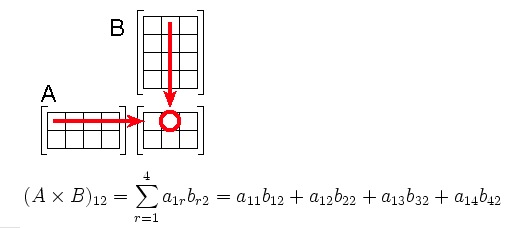
\includegraphics[width=8cm]{figures/matrixProduct.jpg}
\pause \\
\R{$\Q$} is a \B{column} vector. \R{$\P^T$} is a row vector.
%\R{$\P = \angles{ \P(1),\ldots,\P(n) }, \Q = \angles{ \Q(1),\ldots,\Q(m)}$}
\pause \\ ~\\
\R{$\M(\P,\Q) = \P^T \M \Q = \sum_{i=1}^n \sum_{j=1}^m \P(i) \M(i,j) \Q(j)$}
\end{frame}

\section{The basic algorithm}

\begin{frame}
\frametitle{The basic algorithm}
\begin{itemize}
\item Choose an initial distribution \R{$\P_1$}
\item \R{$$\P_{t+1}(i) = \P_{t}(i) {e^{-\eta \M(i,\Qt)} \over Z_t}$$}
\item Where \R{$Z_t = \sum_{i=1}^n \P_{t}(i) e^{-\eta \M(i,\Qt)}$}
\item \R{$\eta>0$} is the learning rate.
\end{itemize}
\end{frame}

\section{The basic analysis}

\begin{frame}
\frametitle{Main Theorem}
\begin{itemize}
\item For \B{any} game matrix $\M$.
\item Any sequence of mixed strat. \R{$\Q_1,\ldots,\Q_T$}
\item The sequence \R{$\P_1,\ldots,\P_T$} produced by \\
basic alg using \R{$\eta>0$} satisfies
\R{\[
   \sumt \mptqt \leq \paren{\frac{1}{1-e^{-\eta}}}\;
        \minp \brac{\eta\; \sumt \mpqt + \RE{\P}{\P_1}}
\]}
\end{itemize}
\end{frame}

\begin{frame}
\frametitle{Corollary}
\begin{itemize}
\item Setting \R{$ \eta = \ln \paren{ 1+\sqrt{\frac{2\ln n}{T}} }$}
\item the average per-trial loss is
\R{\[
   \frac{1}{T} \sumt \mptqt \leq
    \minp \frac{1}{T} \sumt \mpqt + \delt
\]}
\item Where 
\R{\[
\delt = \sqrt{2 \ln n \over T} + {\ln n \over T} 
= O\paren{\sqrt{\frac{\ln n}{T}}}.
\]}
\end{itemize}
\end{frame}

\begin{frame}
\frametitle{Main Lemma}

On any iteration \R{$t$}
\\ ~ \\ \pause
For any mixed strategy \R{$\Pref$}
\\ ~ \\ \pause
\R{$
\RE{\Pref}{\P_{t+1}} - \RE{\Pref}{\P_t} \leq 
\eta \M(\Pref,\Q_t)  - (1-e^{-\eta})\M(\Pt,\Qt)
$}
\end{frame}

\begin{frame}
\frametitle{Visual intuition}

\R{$
\RE{\Pref}{\P_{t+1}} - \RE{\Pref}{\P_t} \leq
\eta \M(\Pref,\Q_t) 
-
(1-e^{-\eta})\M(\Pt,\Qt)
$}
\pause \\ ~ \\ ~ \\
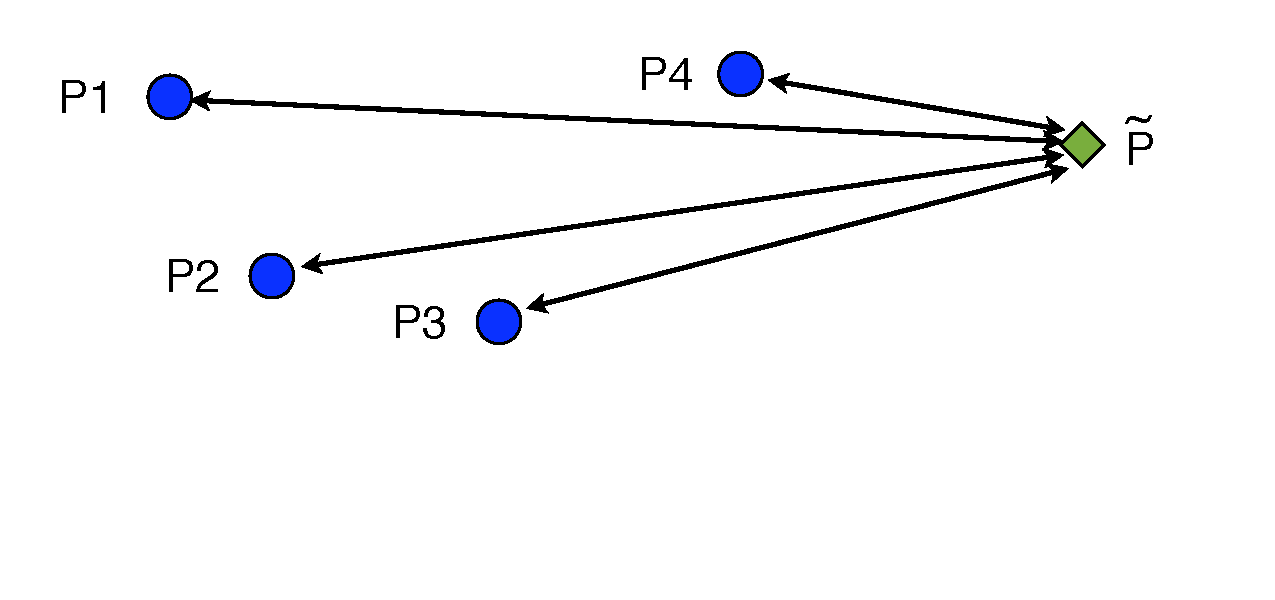
\includegraphics[width=10cm]{figures/divergenceAnalysis.pdf}
\end{frame}

\begin{frame}
\frametitle{Proof of Lemma (1)}
\R{\begin{eqnarray*}
\lefteqn{
\RE{\Pref}{\P_{t+1}} - \RE{\Pref}{\P_t}} \pause \\
&=& 
\sum_{i=1}^n \Pref(i) \ln {\Pref(i) \over \P_{t+1}(i)}
- \sum_{i=1}^n \Pref(i) \ln {\Pref(i) \over \P_t(i)} \pause \\
&=&
\sum_{i=1}^n \Pref(i) \ln {\P_t(i) \over \P_{t+1}(i)}\pause \\
&=&
\sum_{i=1}^n \Pref(i) \ln {Z_t \over e^{\eta \M(i,\Qt)}}
\end{eqnarray*}
}
\end{frame}


\begin{frame}
\frametitle{Proof of Lemma (2)}
\R{\begin{eqnarray*}
&=&
\eta \sum_{i=1}^n \Pref(i) \M(i,\Qt) + \ln Z_t \pause \\
&\leq&
\eta \M(\Pref,\Qt)
+
\ln\brac{\sum_{i=1}^n \P_{t}(i) \left( 1- (1-e^{-\eta}) \M(i,\Qt) \right)}
\pause
\\
&=&
\eta \M(\Pref,\Q_t) 
+
\ln \left( 1-(1-e^{-\eta})\M(\Pt,\Qt) \right)
\pause \\
& \leq &
\eta \M(\Pref,\Q_t)  + (1-e^{-\eta})\M(\Pt,\Qt)
\end{eqnarray*}
}
\end{frame}


\section{Proof of minmax theorem}

\begin{frame}
\frametitle{The minmax Theorem}
~\\
John von Neumann, 1928.
\\ ~ \\ \pause
\R{\[ \minp \maxq \mpq \leq \maxq \minp \mpq \]}
\\ ~ \\ \pause
In words: for \B{mixed} strategies, choosing second gives no advantage.
\end{frame}

\begin{frame}
\frametitle{Proving minmax Theorem using online learning (1)}
~\\
Row player chooses \R{$\P_t$} using learning alg. \\ \pause 
Column player chooses \R{$\Q_t$} \B{after row player} so that
\R{$\Qt = \arg \maxq \mptq$}
\\ \pause
Let \R{$\Pa \doteq \frac{1}{T} \sumt \Pt$} and
\R{$\Qa \doteq \frac{1}{T} \sumt \Qt$}
\\ \pause
\R{\em
\[
\begin{array}{rcll}
{\displaystyle{\minp \maxq \trans{\P}\M\Q}} 
 &\leq&
\displaystyle{\maxq \trans{\Pa}\M\Q} & \nextline
\pause
  &=&
\displaystyle{\maxq \frac{1}{T} \sumt \trans{\Pt}\M\Q}
                       &\mbox{\rm by definition of~~\Pa}\nextline
\pause
  &\leq&
\displaystyle{\frac{1}{T} \sumt \maxq \trans{\Pt}\M\Q} &
\end{array}
\]
}
\end{frame}


\begin{frame}
\frametitle{Proving minmax Theorem using online learning (2)}
\R{\em
\[
\begin{array}{rcll}
  &=&
\displaystyle{\frac{1}{T} \sumt \trans{\Pt}\M\Qt}
                       &\mbox{\rm by definition of~~\Qt}\nextline
\pause
  &\leq&
\displaystyle{\minp \frac{1}{T} \sumt \trans{\P}\M\Qt + \delt}
                       &\mbox{\rm by the Corollary} \nextline
\pause
  &=&
\displaystyle{\minp \trans{\P}\M\Qa + \delt}
                       &\mbox{\rm by definition of~~\Qa}\nextline
\pause
  &\leq&
\displaystyle{\maxq \minp \trans{\P}\M\Q + \delt.} &
\end{array}
\]
}
\pause
but \R{$\delt$} can be set arbitrarily small.

\end{frame}

\begin{frame}
\frametitle{Minmax is weaker than diminishing regret}
\begin{itemize}
\item The minmax theorem proves the existence of an \B{Equilibrium}.
\item Learning guarantees no regret with respect to the past.
\item If all sides use learning, then game will converge to minmax equilibrium.
\item If opponent is not optimally adversarial (limited by knowledge, computationa power...) then learning gives \B{better} performance than min-max.
\item Is it realistic to assume that markets are at equilibrium?
\item If game is not zero sum (allows incentives to collaborate) and all players
use learning then game converges to \B{correlated equilibrium}.
\end{itemize}
\end{frame}

\iffalse %%%%%%%%%%%%%%%%%%%%%%%%%%%%%%%%%%%%%%%%%%%%%%%%%%%%%%%%%%%%%%%%%%

\section{Approximately solving games}

\subsection{Fixed Learning rate}
\begin{frame}
\frametitle{Using average row distribution}
\begin{itemize}
\item XXX
\end{itemize}
\end{frame}

\begin{frame}
\frametitle{Using the average column distribution}
\begin{itemize}
\item XXX
\end{itemize}
\end{frame}

\subsection{Variable learning rate}
\begin{frame}
\frametitle{Using the final row distribution}
\begin{itemize}
\item XXX
\end{itemize}
\end{frame}

\begin{frame}
\frametitle{}
\begin{itemize}
\item XXX
\end{itemize}
\end{frame}

\fi %%%%%%%%%%%%%%%%%%%%%%%%%%%%%%%%%%

\end{document}


